\documentclass[a4paper,12pt]{article}
%\RequirePackage[l2tabu,orthodox]{nag}

\usepackage{upreport}

\title{Evert: A modular time-series analysis environment}
\author{Eduan Oosthuizen}
\studentnumber{13019105}
\subject{CSC 411}
\date{\today}

\begin{document}
\maketitle
\makecoverpage

\pagestyle{plain}
\thispagestyle{plain}
\pagenumbering{roman}

\begin{center}
\LARGE\textbf{\thetitle}
\end{center}

\section*{Synopsis}
The use of Python libraries and JavaScript code allowed for development of a self-contained plotting widget hosted on a local web server that can be accessed with a web browser.

A basic application structure that allows modular expansion of the existing web application was set up using the Flask Python library. Flask allows for use of the Jjinja2 templating engine, incorporating Bootstrap and creating web forms which in combination provided ample resources for a functional and expandable user interface.\\In addition to the widget, the current interface allows for uploading files to the local server.

The Bokeh Python library was used to create the plotting widget. Interactive zooming and panning; multiple axis with associated data sets and an interactive first order fit was accomplished using Bokeh and additional JavaScript code.

Future work includes development of an application structure suited for a large scale application, using an SVG type plot rather than HTML5 canvas and the incorporation of Ajax to perform server side calculations.\newline

\noindent KEYWORDS: EVERT, TIME-SERIES, MODULAR, INFORMATION VISUALISATION

\newpage
\tableofcontents
\newpage
\listoffigures
%\newpage
%\listoftables
\newpage
%\chapter*{Nomenclature}
\printnomenclature
\newpage

\pagestyle{plain}
\setcounter{page}{1}
\pagenumbering{arabic}

\section{Introduction}
Functional computer code developed as part of research projects is often either no longer actively developed or entirely replaced when individuals that initially requested its development, are no longer directly involved with its application. This takes place even though the research findings point to areas of future improvement and investigation.
A possible cause is that software has in many instances been developed with no thought to continued use and development by individuals that are not professional developers. Developing software with easy re-use and active development in mind is a possible solution.

One set of tools that will benefit from collaborative development is a time-series data analysis system.\\The development of such an analysis system, named Evert, is used to explore how an effective platform may be created where engineers can contribute their coded tools to a system of ready-to-use analysis tools.

The Evert project is an ongoing research project within the Process Modelling and Control group at the University of Pretoria's Department of Chemical Engineering. A number of postgraduate and undergraduate students contribute to this project in completion of their degrees.

The research relevant to Evert as an engineering tool and analysis system is presented by \citet{oos_wil}. In this report the process of development is used to find the most effective means in which to create the Evert project for collaborative use.

The development of a single time-series analysis tool was explored using a web application structure. This decision may, however, change as the project continues and more effective means are found outside the web environment.\\The web application approach was chosen as most modern computers such as smart phones, tablets, notebook computers and desktop computers, have a web browser installed irrespective of the operating system. Web applications should therefore exclude the smallest amount of users.

This investigation is authored by an undergraduate engineering student as such a student may be considered relatively inexperienced in web application development. The learning path approximates what could be expected from an engineering professional with similar lack of web application experience.

\section{Theory}
For understanding the development process, basic concepts relevant to the web environment are presented here. Figure~\ref{fig:webpage} shows a web page with inspection of its underlying code in the Google Chrome browser. The web page is displayed on the left and the code inspection window on the right.

\begin{figure}[htbp]
  \centering
  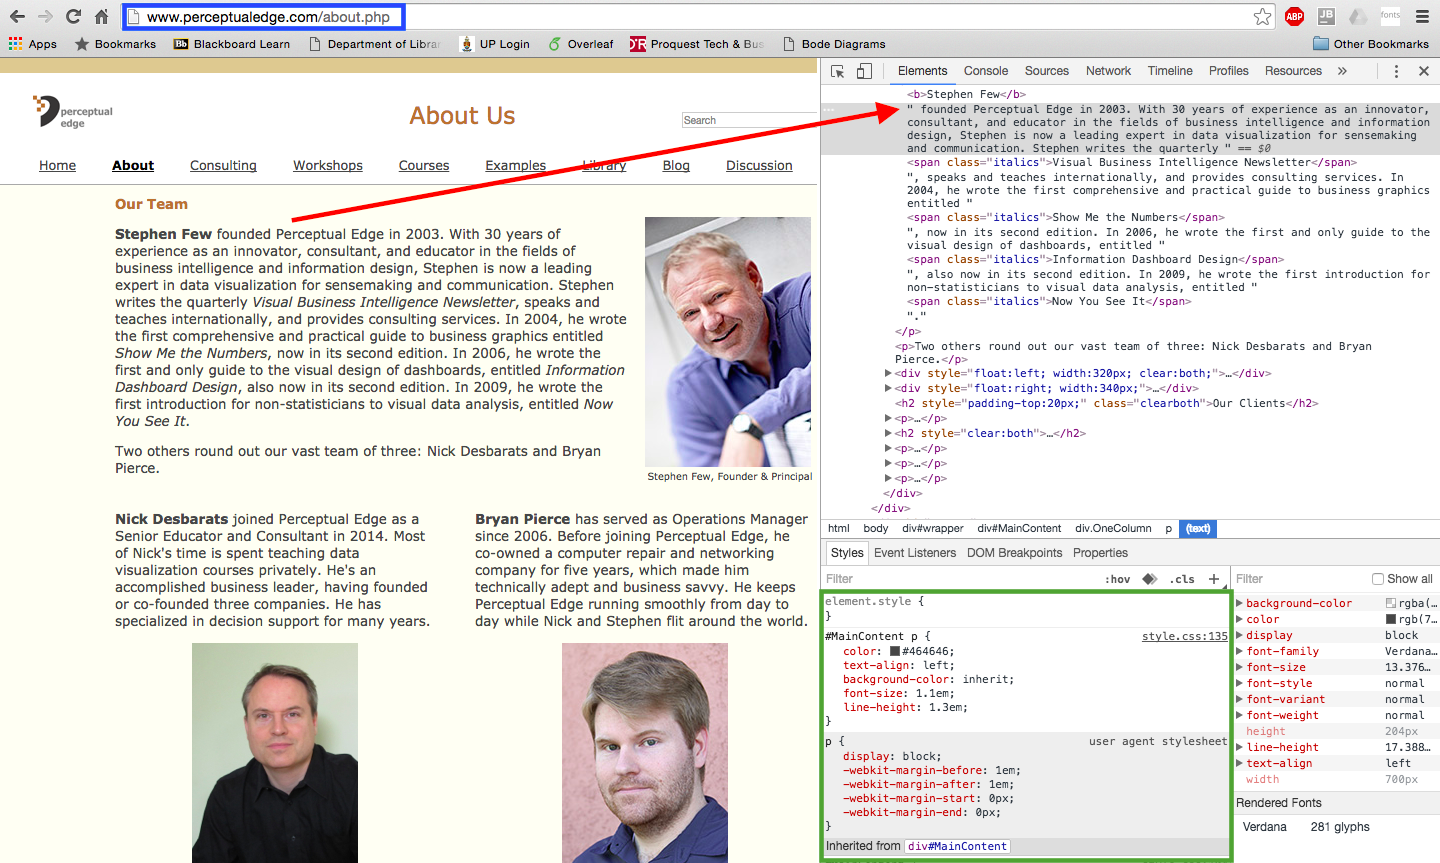
\includegraphics[width=\textwidth]{webpage.png}
  \caption[Web page with inspection of code]{Web page with underlying code inspection in the Google Chrome web browser}
  \label{fig:webpage}
\end{figure}

Web browsers, such as Microsoft Edge, Mozilla Firefox and Google Chrome, are computer programs that supply a graphical user interface (GUI) for users to explore content served on the internet \citep{itl}.\\The files that are referred to here are sets of instructions to the browser to correctly display the web page. The file types relevant here are HTML, CSS and JavaScript.

HTML is an initialism for Hypertext Markup Language which is a web standard. This programming language allows for the creation of structured documents for the web by using a document object model (DOM) of page elements generated and displayed by the browser \citep{larsen}. These page elements are represented by \emph{tags} in the HTML text.\\Figure~\ref{fig:webpage} shows a web page on the left with its source code displayed in an inspection window on the right. The red arrow points from a web page element to its corresponding HTML tag.\\The current version of this web standard, HTML5, allows for the development of cross-platform user interfaces which include the mobile and web platforms \citep{larsen}.

Each DOM element can be styled using a web standard called CSS which is an initialism for Cascaded Style Sheets \citep{larsen}. This code can be added either in the page element's HTML tag or by using a separate file that contains the styling code.\\HTML specifies only the layout of a web page and CSS the style of each of its elements.\\The green rectangle in Figure~\ref{fig:webpage} shows the CSS relevant to the web page.

JavaScript is a computer programming language created by Brendan Eich that is currently supported by all common web browsers \citep{rauschmayer}. JavaScript may be used like any other programming language like Python, Java or Visual Basic. Its relevance to web applications is due to how it has been integrated into the web environment and has led to, for example, HTML tags having \emph{on-click events}. When a user \emph{clicks} on an HTML tag rendered as a DOM element the on-click event calls a JavaScript script which is executed by the web browser \citep{rauschmayer}.\\The functionality of JavaScript that will be exploited is its integration for an HTML constructed GUI.

For the design of components that are reusable across different web pages the HTML, CSS and JavaScript can be combined into what is referred to as a widget \citep{snoyman}.

For displaying plots in web pages one of two DOM elements can be used: \emph{canvas} or \emph{SVG}.\\A canvas element draws what is being displayed pixel-by-pixel by using JavaScript code. This element makes out part of the DOM, but whatever is drawn on it, does not. Any change in the image that is being rendered results in the entire image being regenerated.\\For an SVG element, however, every shape is an element in the DOM of the web page and can therefore be accessed and changed using modular JavaScript code, changing only that single element within and not the rest of the SVG element \citep{svgCanvas}.

%As a note to self- Berners is the correct spelling.
The internet, or web, as it is known today was sparked in a proposal by Tim Berners-Lee, an English scientist at the particle physics research institute CERN \citep{lubanovic}. Bernes-Lee set three functionalities for the design of the web: HTTP, HTML and URL.\\HTTP is an initialism for Hypertext transfer protocol, which is the name of the specification used by web clients and servers to exchange requests and responses. \\URL is an initialism for Uniform Resource Locator which is how each resource (web page or file) on the web is uniquely represented. In common speech this is referred to as the web address of some internet resource and is shown by the blue rectangle in Figure~\ref{fig:webpage}.\\Each of these standards have a vast number of supporting technologies, but such detail is not necessary in this text.

Figure~\ref{fig:clientServer} shows an illustration of how web \emph{clients} and \emph{servers} interact when a client requests a resource.\\A web client sends a request to a web server by opening a channel for data transmission and sending the URL to the server. The server then responds by sending back the relevant data located at the requested URL \citep{lubanovic}.\\This is referred to as the client-server model of the web.

\begin{figure}[htbp]
  \centering
  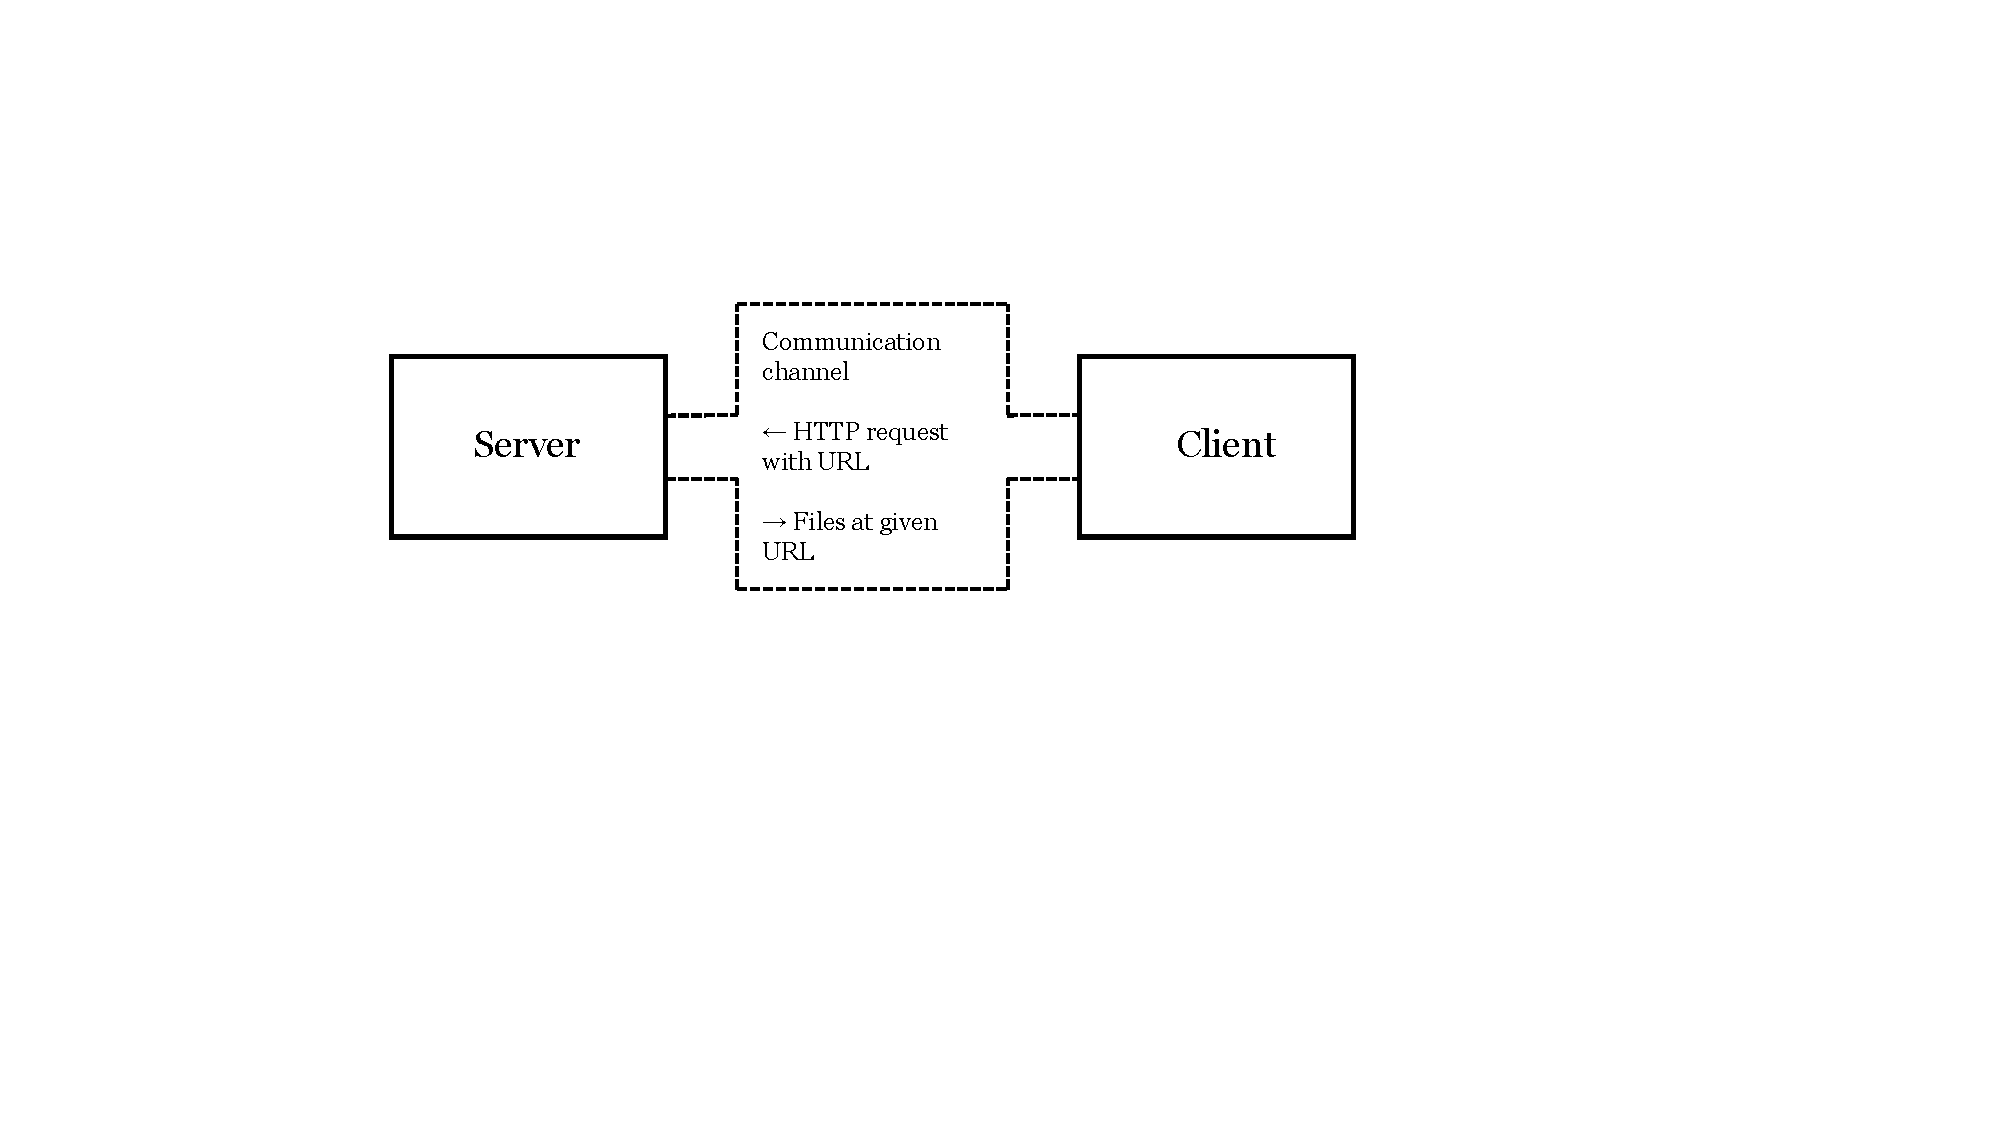
\includegraphics[width=\textwidth]{clientServer.pdf}
  \caption[Client-server model]{Illustration of the client-server model of the web}
  \label{fig:clientServer}
\end{figure}

\section{Development of an application structure and widget for Evert}
A widget that allows the user to interactively fit a first order response curve to a single data set was developed and is shown in Figures~\ref{fig:widget_overview_neutral} to~\ref{fig:widget_overview_select}. The widget also allows for interactive zooming, panning and plotting of multiple data sets using multiple axes.\\The theory in support of such an analysis tool is explored by \citet{oos_wil}.

The source code of the widget is available in the following web repository: \url{https://github.com/Eduan-Oosthuizen/Evert_2016.git}

The plotted data sets exploit the pre-attentive attribute of colour to let users differentiate between each data set without cognitive thought \citep{oos_wil}.

\begin{figure}[htbp]
  \centering
  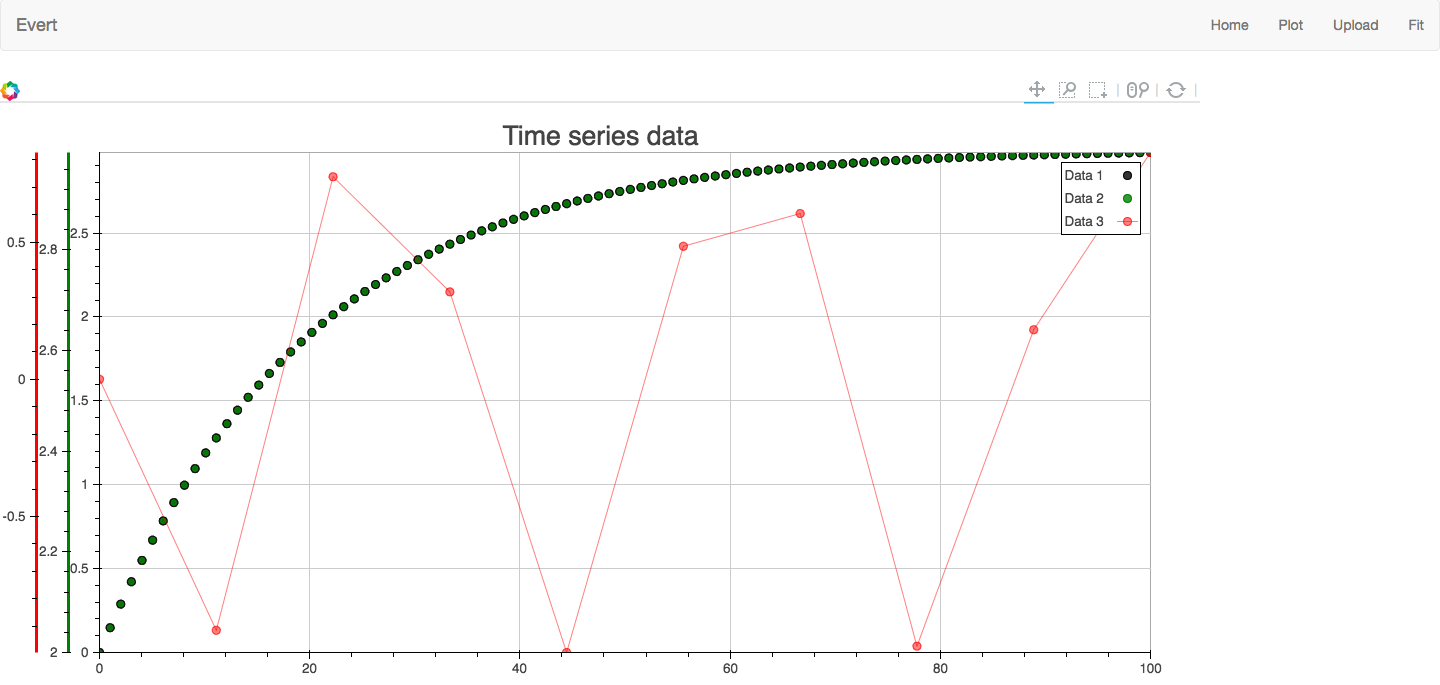
\includegraphics[width=\textwidth]{widgetNeutral.png}
  \caption[Neutral first-order fit widget]{Screen shot of the neutral first-order fit widget}
  \label{fig:widget_overview_neutral}
\end{figure}

\begin{figure}[htbp]
  \centering
  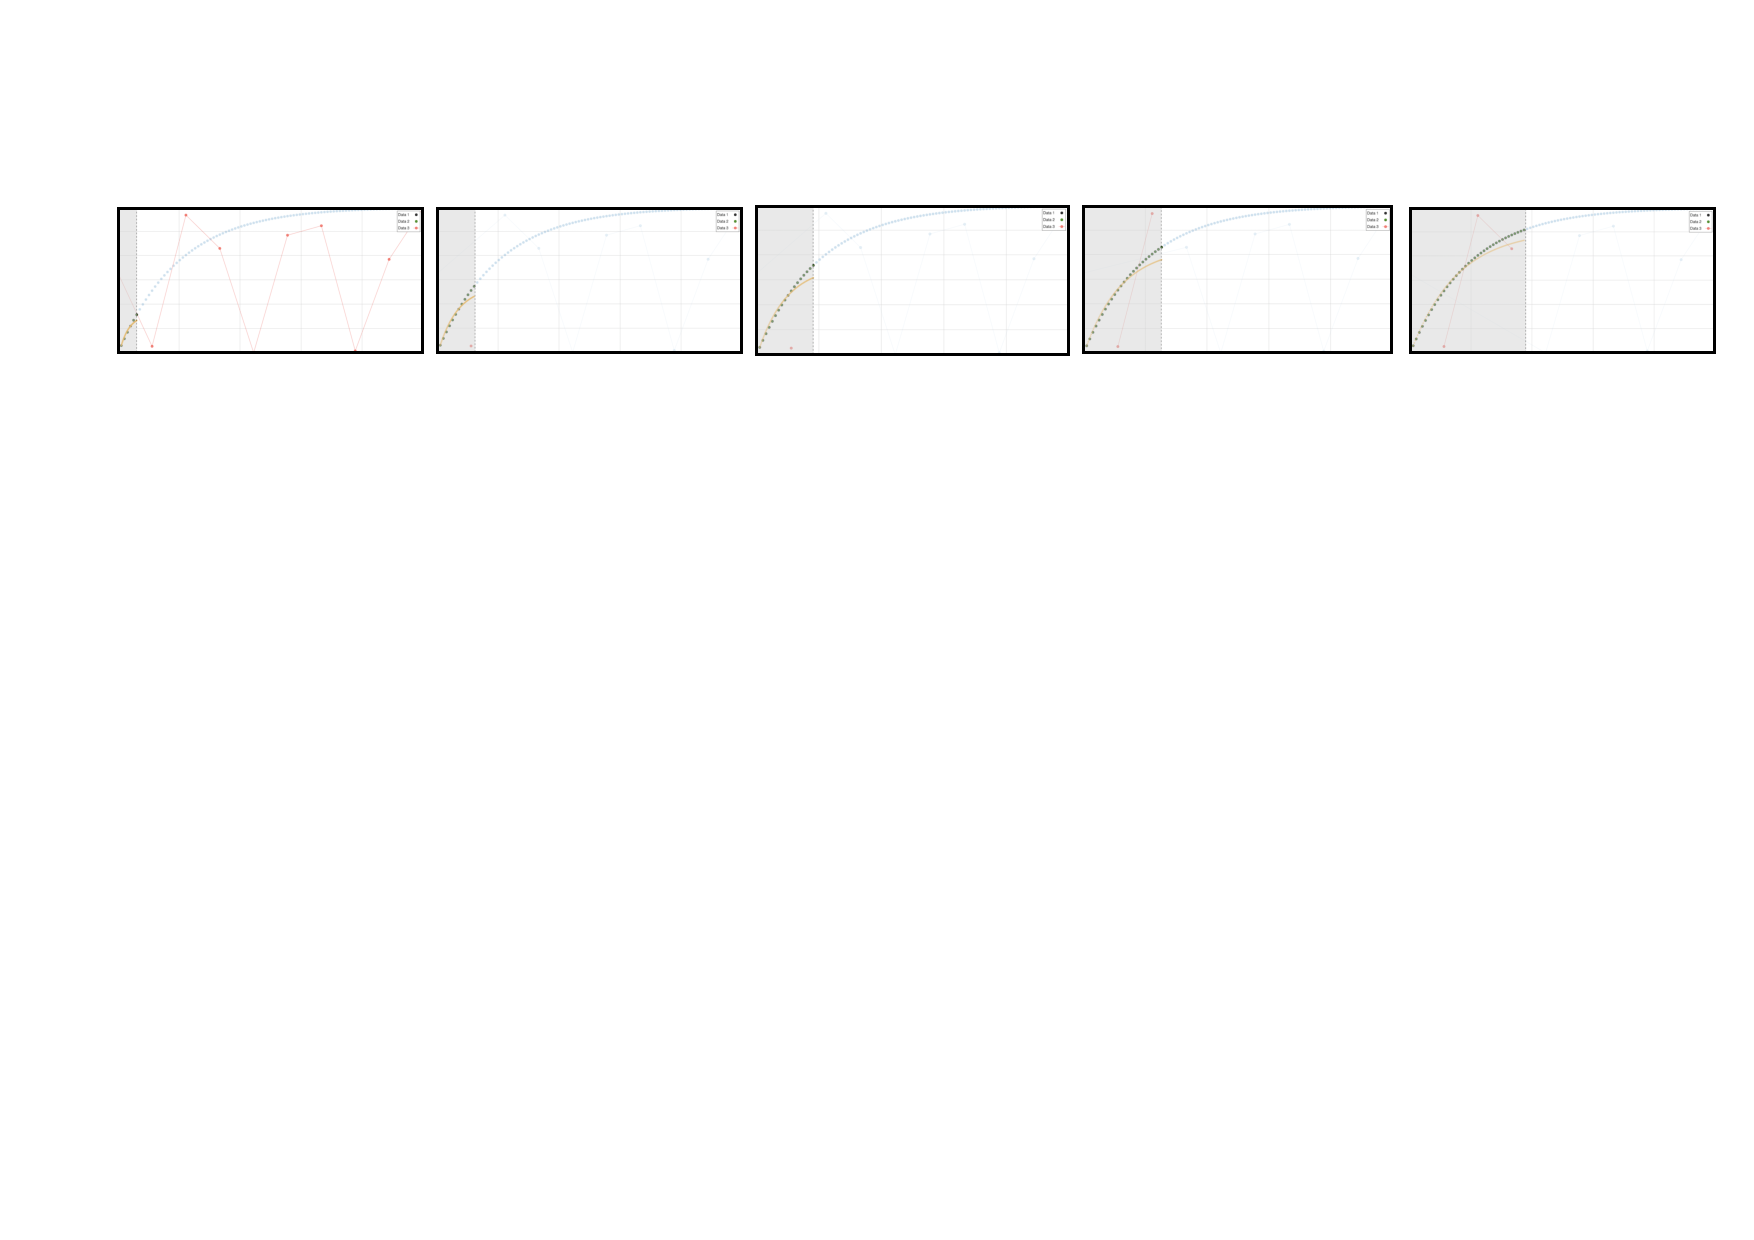
\includegraphics[width=\textwidth]{smallMultiples.pdf}
  \caption[Small multiples of interactive fit response]{Small multiples of the active interactive first-order fit widget showing widget behaviour while fit is performed}
  \label{fig:widget_smallMultiples}
\end{figure}

\begin{figure}[htbp]
  \centering
  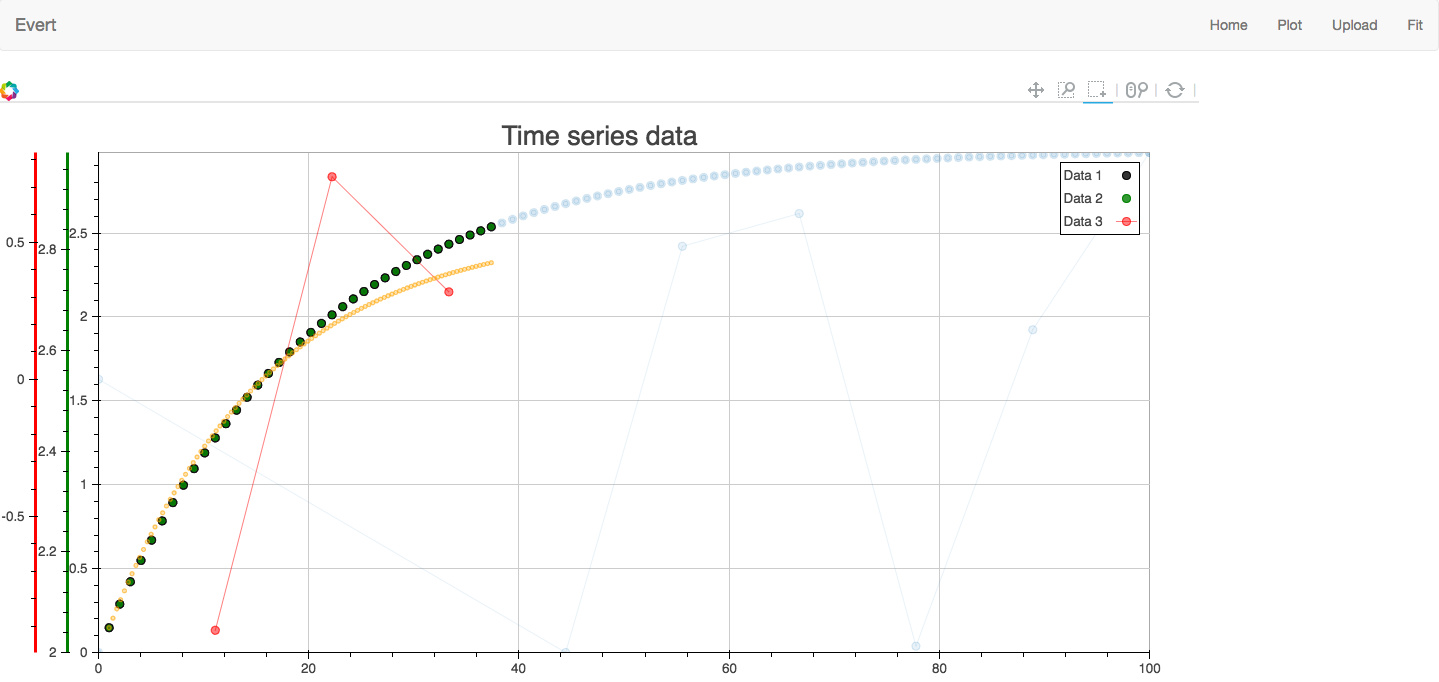
\includegraphics[width=\textwidth]{widgetFit.png}
  \caption[Active first-order fit widget]{Screen shot of the active first-order fit widget after mouse release}
 \label{fig:widget_overview_select}
\end{figure}

\subsection{Interaction of different libraries}
Figure~\ref{fig:libraries} shows a schematic diagram of the interaction between different libraries and elements of the current Evert system as a guideline for the remainder of this section.

\begin{figure}[htbp]
  \centering
  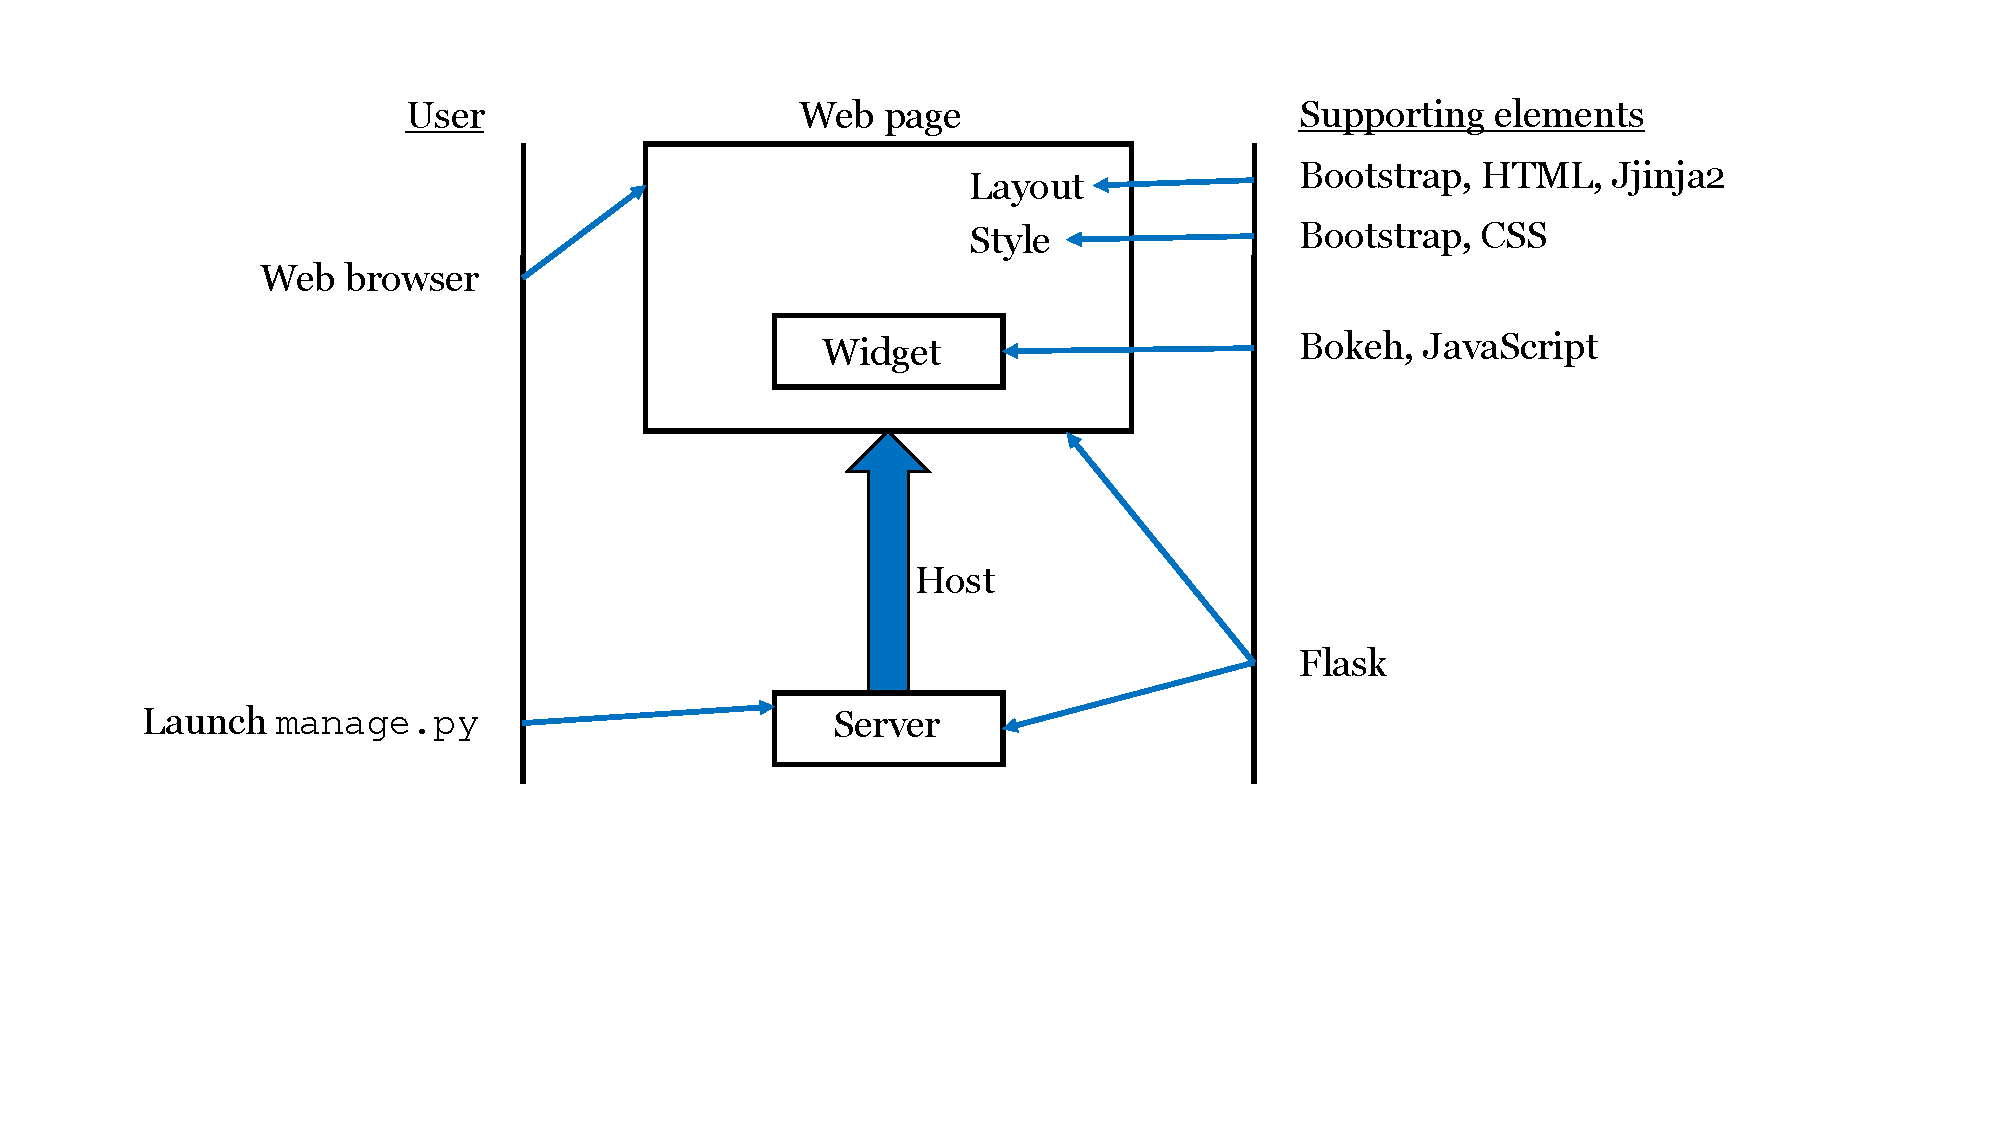
\includegraphics[width=\textwidth]{systems.pdf}
  \caption[Programming library interaction an user view]{Illustration showing the supporting libraries for the elements of the web application and how the user interacts with the application.}
  \label{fig:libraries}
\end{figure}

From the point of view of the end user of the Evert system the application is launched by executing the Python script named \texttt{manage.py} and using a web browser to access the locally hosted web site.\\The role of each of the supporting elements listed on the right of Figure~\ref{fig:libraries} is discussed in detail in the remainder of this section.

\subsection{Local web server and application structure}
A local web server was created using the Flask library in the Python programming language \citep{flask}. Flask provides a framework for developing web applications that are modular by using what is called an application blueprint. These functionalities were implemented as shown by \citet{grinberg}.

The application is initialised in a given directory as an object in the Python programming language. The local server is also created in this directory and all the relevant Python code is executed by the server. There are two directories that make up part of the structure that should be noted: \texttt{app} and \texttt{static}.

Python files in the \texttt{app} directory allow for web pages to be added to the application by editing either the \texttt{views.py} or \texttt{error.py} file. From \texttt{views.py} all web pages, apart from error handling pages, will be rendered. Error handling pages are rendered from the \texttt{errors.py} file when error codes are generated by the server.\\As the relevant URLs are passed to the server as HTTP requests the application object executes the correct Python function that is responsible for rendering the requested page.

The \texttt{static} directory is recognized by the application object as the directory in which all static files needed for the web application are stored. Examples of these files are the JavaScript file that includes the code for the first order response fit, CSS files and all necessary HTML files that store the layouts of each web page.

As the Python programming language had been chosen for server-side programming the Flask library was found to serve the purpose of not only allowing for a local web server to be deployed, but also providing an application layout framework, access to the Jjinja2 web framework and also use of Bootstrap and creation of web forms \citep{flask}.\\To illustrate some of these functionalities a web page was added to the application that allows for uploading files to the \texttt{static} directory from a web browser. Navigation between web pages is possible by use of a navigation bar.

For the layout of the content in web pages, Flask uses the Jjinja2 template engine \citep{jjinja2}. In conjunction with developing all HTML files using Jjinja2, the Flask-Bootstrap extension was also used to allow for easy integration of the Bootstrap client-side web framework \citep{grinberg}. Bootstrap provides a library of user-interface components that allow for clean and responsive web pages. In the current version of the Evert application the navigation bar is one such component.

For contributors that have only used a GUI in using computers the above steps will require some exposure to how file navigation takes place using a PATH for locating resources in the \texttt{static} directory.

These steps took up the majority of time for the development process.

\subsection{Generating an interactive plotting widget using Bokeh}
To generate the interactive plotting widget that performs the first order response fit the Bokeh Python library was used \citep{bokeh}. In using Bokeh all the desired functionality of the plotting widget is specified in the relevant Python function that represents the web page housing the widget. Bokeh then generates a populated HTML \emph{div} tag and a JavaScript function as an HTML \emph{script} tag that is called by the \emph{div} tag. These HTML tags are passed as variables to the Jjinja2 template that is rendered for the web page. The result is the widget displayed in  Figures~\ref{fig:widget_overview_neutral} and~\ref{fig:widget_overview_select}.\\The plotting widget's web page is accessed by using the navigation bar.

Each of the functionalities provided by this widget are standard components of the Bokeh library.\\Each data set is passed to the Bokeh function that generates the HTML tags as a Python object. The data object employed in the Evert widget allows for JavaScript code to be added to it as code that is executed by the web browser whenever the data is selected. The necessary JavaScript function to perform the first order fit is loaded from the \texttt{static} directory by the HTML template for the web page upon rendering. The JavaScript function name is passed to the callback property of the data object.\\The callback execution was also set to take place for every change in selection of the data so that the fit is performed dynamically without the user releasing the mouse.

The DOM element that is rendered by the Bokeh HTML \emph{div} tag is an HTML5 canvas \citep{bokeh}. Any interaction with plot elements from JavaScript code not passed to Bokeh as a callback function upon creation of the canvas element can therefore not manipulate the plot.

\section{Discussion of modular approach}
Evert is designed as a modular system to allow contribution of new tools and academic projects within the field of time-series data analysis, the system should provide a framework that is easy to use.

Assuming that a potential contributor is familiar with the Python language, the use of Bokeh to generate interactive plots proved simple.\\The creation of the web application framework and a web page to house the widget, however, necessitates the use of more complicated constructs in the Python language as well as HTML and Jjinga2 for basic functionalities. Custom functionalities require the addition of JavaScript code to be passed to Bokeh in generating the HTML5 canvas element.

Concerning the addition of more advanced functions, which are currently not available in Bokeh, the use of an SVG element rather than canvas in the DOM will be beneficial.\\An SVG element's constituting elements can easily be accessed and manipulated using JavaScript and the D3.js library after creation of the element and its layout.

Distribution of the Evert project with the option of using any of number of available plotting libraries might be a viable option to allow contributors to use whichever library they are familiar with. Such an approach might not, however, allow for consistency in layout.

\section{Future work}
The rendering of the widget as an HTML5 canvas element restrains the amount of custom interaction that can be added using JavaScript, one such example is the addition elements to the plot after the page has been rendered- such as text annotations that follow the mouse pointer and become invisible when the pointer leaves the SVG element.\\Adding similar functionalities using Bokeh is only possible when they are added to the standard Bokeh library objects and functions.

Creating plots that consist of SVG elements is possible using a JavaScript library called D3.js or one of two Python libraries- Plotly and mplD3 \citep{d3, plotly, mpld3}.

Investigation of these libraries may prove one of them to be more suited for use in Evert.

An investigation into the basic use of D3.js showed that the use of this library is considerably more complex when compared to Bokeh.\\It should be possible to use one of the Python libraries to generate the SVG element and its contents upon rendering the web page and then add advanced functionalities using D3.js. The confirmation of this is also left to future research.

Optimal application structure for large scale projects should be further investigated to allow for growth in size and complexity of the Evert system. The current structure may not be adequate for a large web application.

The use of JavaScript for calculations on the client side of the web application may not be optimal and the Ajax set of technologies should be investigated.\\Ajax allows for web resources to be requested without the web page being reloaded \citep{powers}. The use of Ajax in the Evert web application could be to use Python scripts that run on the server side to do calculations, such as a first order fit. Only the fit parameters or a list of data points that need to be plotted are returned to the client side.

\section{Conclusions and Recommendations}
The exclusive use of Python libraries and JavaScript allowed for successful development of a self-contained widget hosted on a local server that can be accessed using a web browser.

Using a basic Flask application structure modular expansion of the existing web application was made possible. As the project grows in size it is recommended that this structure be changed for optimal performance.\\Flask also allows for use of the Jjinja2 templating engine, incorporating Bootstrap and creating web forms which in combination provide ample resources for a functional and expandable user interface.\\The current interface allows for uploading files to the local server and using the created widget. Each of these functionalities are placed on different web pages accessed via a navigation bar.

The development of the widget using Bokeh proved simple. Interactive zooming and panning; multiple axis with associated data sets and an interactive first order fit was accomplished using Bokeh and additional JavaScript code.\\Future work in finding an SVG generating library rather than canvas, as with Bokeh, is recommended to allow for functionality to be added using JavaScript functions not passed to the Python library used in creating the initial widget content.

Recommended future work includes development of an application structure suited for a large scale application as well as the incorporation of Ajax to perform server side calculations.

\bibliography{report}
\bibliographystyle{chemeng}

\end{document}